\chapter{Dynamic Transport Services}
\label{ch:dts}
% ##################################################################################################################

\hfill \textbf{Author:} Michal Maciejewski

\begin{center} 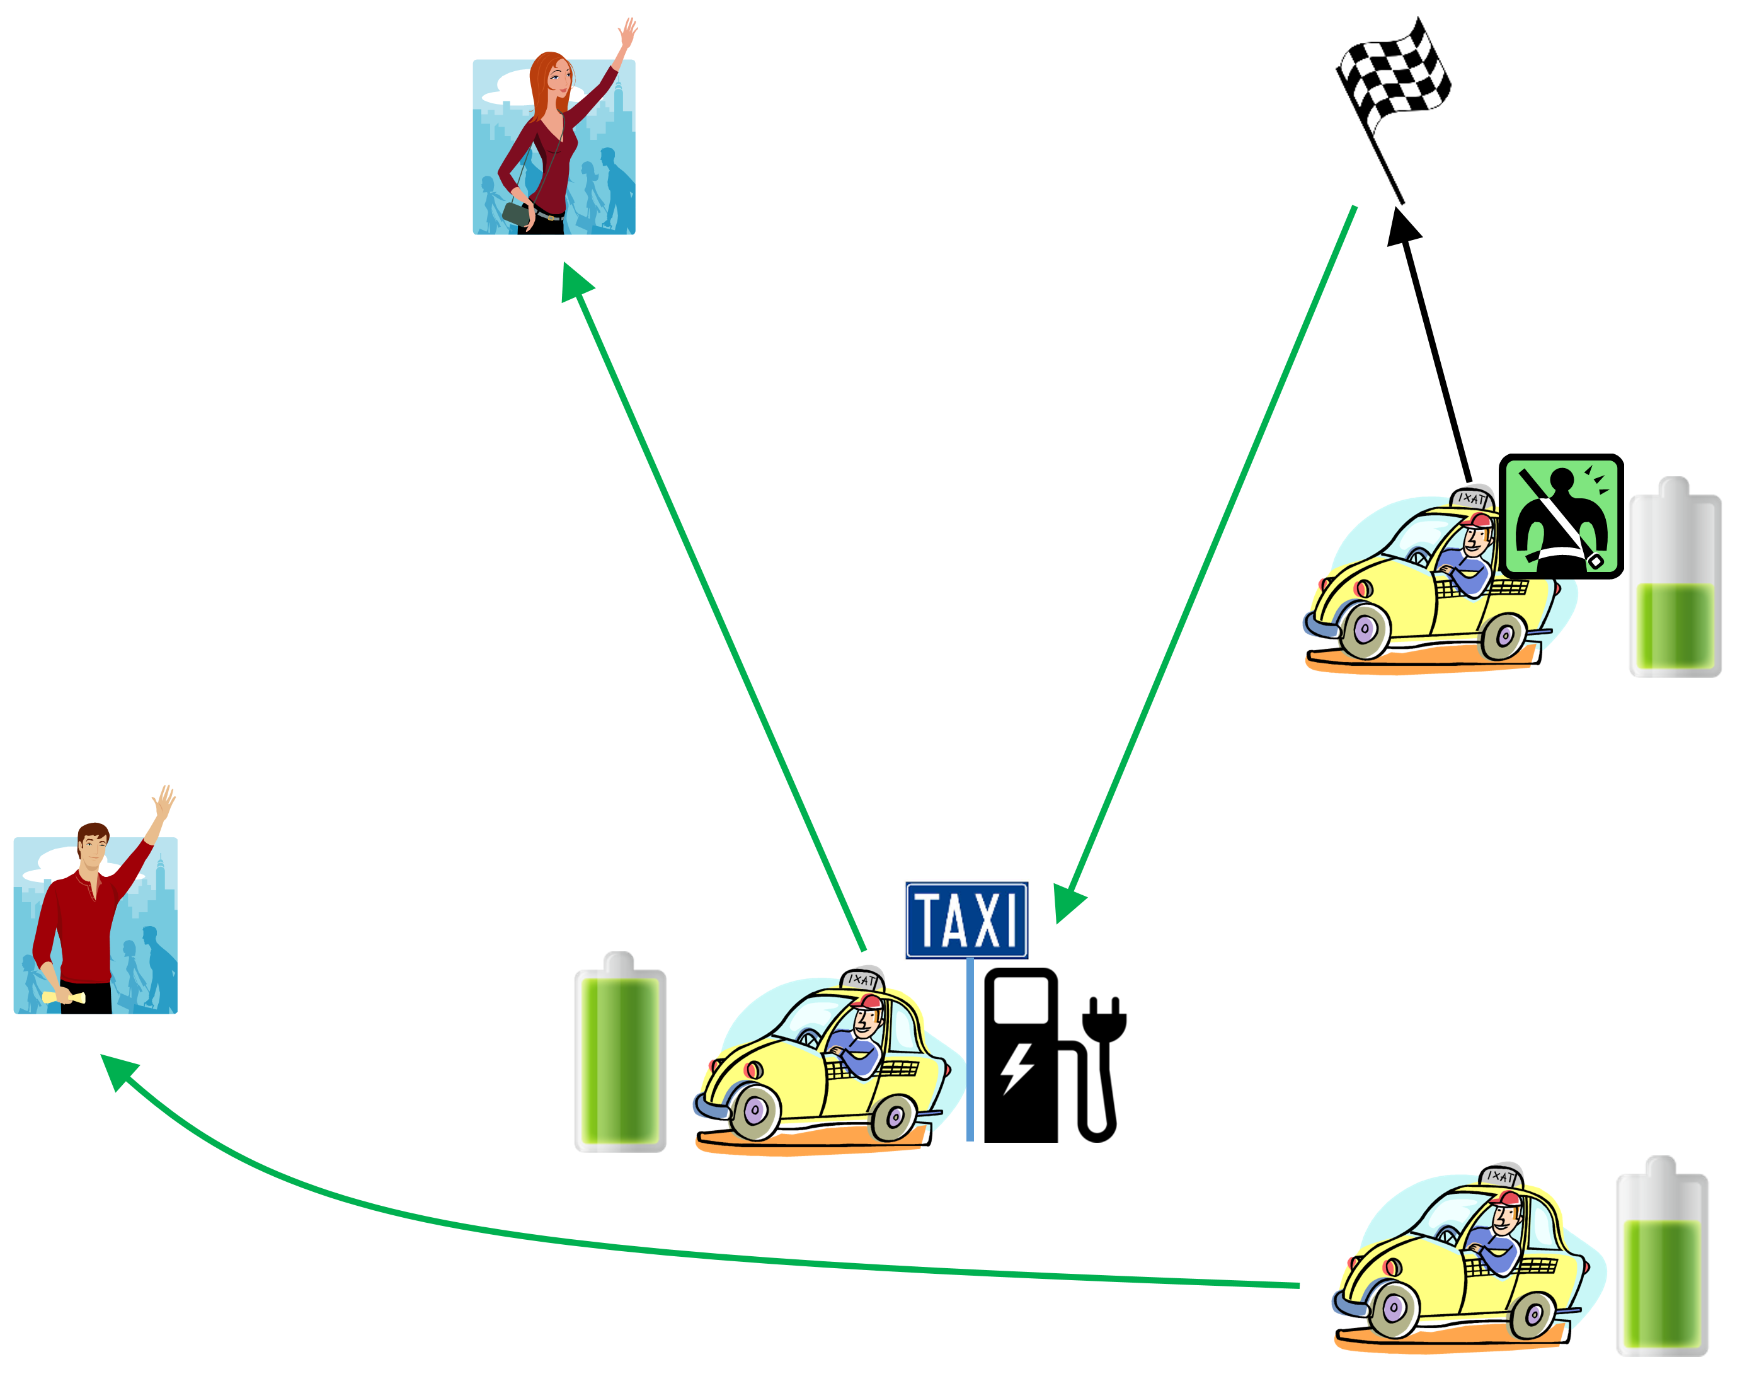
\includegraphics[width=0.67\textwidth, angle=0]{extending/figures/DTS/eTaxiDispMatsimBook.png} \end{center}

\editdone{This text has undergone the professional edit. Please no grammatical changes anymore! They are most-probably wrong.}

% ##################################################################################################################
\section{Basic Information}
\createStandardInformationBasic{\url{http://matsim.org/javadoc} $\to$ core $\to$ vrp}{No predefined invocation. Setting up a \lstinline|VrpOptimizer| and coupling it with \gls{matsim} requires some tailor-made code as shown in Section~\ref{sec:dvrp_config}. A starting point is \lstinline|RunOneTaxiExample|.}{No typical \gls{matsim} config}
{
\citet{MaciejewskiNagelOnlineTaxis2, MaciejewskiNagel2013OnlineTaxisVSPWP, MaciejewskiNagel2013CooperationPPAM, Maciejewski2014OnlineViaOffline}
}

\kai{@Joschka: Würde mir für obiges noch folgendes wünschen: (1) Verwendung von createStandardInformation ohne ``basic''. (2) Ein Skript-in-Java mit Namen ``RunXxx''.}
\joschka{(1) ist wegen der Nicht-Verwendung von configs etwas schwierig. (2) ist eingebaut}
\kai{Joschka, Können wir es nicht zum Anlass nehmen, dem dvrp mal eine normale config zu verpassen?  Schau mal bei RoadPricing.  Ist aber nicht so kritisch; eine RunXxx-Klasse ist schonmal deutlich besser als gar nichts.}
\joschka{Kai, siehe Mails mit Michal - ist in Arbeit.}

% ##################################################################################################################
\section{Introduction}
The recent technological advancements in \gls{ict} provide novel, on-line fleet management tools, opening up a broad range of possibilities for more intelligent transport services: flexible, demand-responsive, safe and energy/cost efficient. Significant enhancements can aid in both traditional transport operations, like regular public transport or taxis and introduction of novel solutions, such as demand-responsive transport or personal rapid transport. However, the growing complexity of modern transport systems, despite all benefits, increases the risk of poor performance, or even failure, due to lack of precise design, implementation and testing.

One solution is to use simulation tools offering a wide spectrum of possibilities for validating transport service models. Such tools have to model, in detail, not only the dynamically changing demand and supply of the relevant service, but also traffic flow and other existing transport services, including mutual interactions/relations between all these components. Although several approaches have been proposed \citep[e.g.,][]{ReganMahmassaniJaillet1998DynamicFleetManagementSimulation, BarceloEtc2007RoutingSchedulingSimulationLogistics, LiaoEtc2008ObjOrFramework4DVRP,Certicky:2014:AST:2615731.2616118}, as far the author knows, no existing solutions provide large-scale microscopic simulation that include all the components above.

% ##################################################################################################################
\section{DVRP Contribution}
To address the problem above, \gls{matsim}'s \gls{dvrp} \gls{contribution} has been developed. The \gls{contribution} is designed to be highly general and customizable to model and simulate a wide range of dynamic vehicle routing and scheduling processes. Currently, the domain model is capable of representing a wide range of one-to-many and many-to-many \glspl{vrp}; one can easily extend the model even further to cover other specific cases (see Section~\ref{sec:DVRP_model}). Since online optimization is the central focus, the \gls{dvrp} contribution architecture allows plugging in of various algorithms. At present, there are several different algorithms available, among them a memetic \ah{???} algorithm for the \emph{Dynamic Multi-Depot Vehicle Routing Problem with Time Windows and Time-Dependent Travel Times and Costs}, analyzed in \citep{MaciejewskiNagel2012DVRPMatsimPPAM}, and a family of algorithms for online taxi dispatching, studied in \citep{ MaciejewskiNagelOnlineTaxis2, MaciejewskiNagel2013OnlineTaxisVSPWP, MaciejewskiNagel2013CooperationPPAM, Maciejewski2014OnlineViaOffline}.

The \gls{dvrp} contribution models both supply and demand, as well as optimizing fleet operations, whereas \gls{matsim}'s core is used for simulating supply and demand, both embedded into a large-scale microscopic transport simulation. In particular, the contribution is responsible for:
%
\begin{itemize}\styleItemize
	\item Modeling the \gls{dvrp} domain.
	\item Listening to simulation events.
	\item Monitoring the simulation state (\eg movement of vehicles).
	\item Finding least-cost paths.
	\item Computing schedules for drivers/vehicles.
	\item Binding drivers' behavior to their schedules.
	\item Coordinating interaction/cooperation between drivers, passengers and dispatchers.
\end{itemize}

Dynamic transport services are simulated in \gls{matsim} as one component of the overall transport system. The optimizer plugged into the \gls{dvrp} contribution reacts to selected events generated during simulation, which could be: request submissions, vehicle departures or arrivals, etc. Additionally, it can monitor the movement of individual vehicles, as well as query other sources of online information, \eg current traffic conditions. In response to changes in the system, the optimizer may update drivers' schedules, either by applying smaller modifications or re-optimizing them from scratch. Drivers are notified about changes in their schedules and adjust to them as soon as possible, including immediate diversion from their current destinations. For passenger transport, such as taxi or demand-responsive transport services, interactions between drivers, passengers and the dispatcher are simulated in detail, including calling a ride or picking up and dropping off passengers.

% ##################################################################################################################
\section{DVRP Model}
\label{sec:DVRP_model}
The \gls{dvrp} contribution can be used for simulating \emph{Rich VRPs}. Compared to the classic \emph{Capacitated VRP}, the major model enhancements are:
%
\begin{itemize}\styleItemize
	\item One-to-many (many-to-one) and many-to-many topologies
	\item Multiple depots
	\item Dynamic requests
	\item Request and vehicle types
	\item Time windows for requests and vehicles
	\item Time-dependent stochastic travel times and costs
	\item Network-based routing (including route planning, vehicle monitoring and diversion)
\end{itemize}
%
Except for the travel times and costs (discussed in Section~\ref{sec:VRP-router}), which are calculated on demand, all the \gls{vrp}-related data are accessible via \lstinline$VrpData$.%
\footnote{
Package \lstinline$org.matsim.contrib.dvrp.data$.
}
In the most basic setup, there are only two types of entities, namely \lstinline$Vehicle$s and \lstinline$Request$s. This model, however, can be easily extended as required. For instance, for an electric vehicle fleet, specialized \lstinline$ElectricVrpData$ also stores information about \lstinline$Charger$s. This, and other examples of extending the base \gls{vrp} model, such as a model of the \emph{\gls{vrp} with Pickup and Delivery}, are available in the \lstinline$org.matsim.contrib.dvrp.extensions$ package.

% ========================================================================================
\subsection{Schedule}
\label{sec:VRP-schedule}
Each \lstinline$Vehicle$ has a \lstinline$Schedule$, a sequence of different \lstinline$Task$s, such as driving from one location to another (\lstinline$DriveTask$), or staying at a given location (\eg serving a customer or waiting;  \lstinline$StayTask)$.%
\footnote{
Package \lstinline$org.matsim.contrib.dvrp.schedule$.
}
A \lstinline$Schedule$ is where supply and demand are coupled. All schedules are calculated by an online optimization algorithm (see Section~\ref{sec:VRP-optimizer}) representing the fleet's dispatcher. Each task is in one of the following states (defined in the \lstinline$Task.TaskStatus$ enum): \lstinline$PLANNED$, \lstinline$STARTED$ or \lstinline$PERFORMED$; each schedule's status is one of the following:
%
\begin{itemize}
	\item \lstinline$UNPLANNED$---no tasks assigned
	
	\item \lstinline$PLANNED$---all tasks are \lstinline$PLANNED$ (none of them started)
	
	\item \lstinline$STARTED$---one of the tasks is \lstinline$STARTED$ (this is the schedule's \lstinline$currentTask$; the preceding tasks are \lstinline$PERFORMED$ and the succeeding ones are \lstinline$PLANNED$)
	
	\item \lstinline$COMPLETED$---all tasks are \lstinline$PERFORMED$
\end{itemize}
%
In general, when modifying a \lstinline$Schedule$, one can freely change and rearrange the planned tasks; those performed are considered to be read-only. For the current task, one can, for instance, change its end time, although the start time must remain unchanged. Proceeding from the current task to the next one is carried out by invoking the \lstinline$Schedule.nextTask()$) method.

The execution of the current task may be monitored with a \lstinline$TaskTracker$.%
\footnote{
Package \lstinline$org.matsim.contrib.dvrp.tracker$.
}
In the most basic version, trackers predict only the end time of the current task. More complex trackers also provide detailed information on the current state of task execution. \lstinline$OnlineDriveTaskTracker$, for example, offers functionality similar to GPS navigation, such as monitoring the movement of a vehicle, predicting its arrival time and even diverting its path.

\lstinline$ScheduleImpl$, along with \lstinline$DriveTaskImpl$ and \lstinline$StayTaskImpl$, is the default implementation of \lstinline$Schedule$ and offers several additional features, such as data validation or automated task handling. It also serves as the starting point when implementing domain-specific schedules or tasks (\eg \lstinline$ChargeTask$ in the electric VRP model mentioned above).

\subsection{Least-cost Paths}
\label{sec:VRP-router}

\gls{matsim}'s network model consists of nodes connected by one-way links. Because of the queue-based traffic flow simulation (Section~\ref{sec:trafficflowmodel}), a link is the smallest traversable element (\ie a vehicle cannot stop in the middle of a link). Besides links, the \gls{dvrp} contribution also operates on a higher level of abstraction: paths. Each path is a sequence of links to be traversed to get from one location to another in the network, or more precisely, from the end of one link end to the end of another link. 

The functionality of finding least-cost paths is available in the \lstinline$org.matsim.contrib.dvrp.router$ package. \lstinline$VrpPathCalculator$ calculates \lstinline$VrpPath$s by means of the least-cost path search algorithms available in \gls{matsim}'s core
\citep{JacobMaratheEtAl1999computationalstudyof,LefebvreBalmer_unpub_STRC_2007}.% 
\footnote{
Package \lstinline$org.matsim.core.router$.
}
Because of changing traffic conditions, paths are calculated for a given departure time. Since \gls{matsim} calculates average link travel time statistics for every 15\,minutes time period by default, the 15\,minutes time bin is also used for computing shortest paths.

\lstinline$VrpPath$s are used by \lstinline$DriveTask$s to specify the link sequence to be traversed by a vehicle between two locations. It is possible to divert a vehicle from its destination by replacing the currently followed \lstinline$VrpPath$ with a \lstinline$DivertedVrpPath$.

To reduce computational burden, the already calculated paths can be cached for future reuse (see \lstinline$VrpPathCalculatorWithCache$). However, when calculating least-cost paths from one location to many potential destinations, a significant speed-up can be achieved by means of least-cost tree search (see \lstinline$org.matsim.utils.LeastCostPathTree$).

% ##################################################################################################################
\section{DynAgent}
\label{sec:dynAgent}
Contrary to the standard day-to-day learning in \gls{matsim} (but see also Section~\ref{sec:transients-vs-learning}), in the \gls{dvrp} contribution, each driver behaves dynamically and follows orders coming continuously from the dispatcher. The \lstinline$DynAgent$ class, along with the \lstinline$org.matsim.contrib.dynagent$ package, provides the foundation for simulating dynamically behaving agents. Although created for DVRP contribution needs, \lstinline$DynAgent$ is not limited to this context and can be used in a wide range of different simulation scenarios where agent dynamism is required.

\lstinline$DynAgent$'s main concept assumes an agent can actively decide what to do at each simulation step instead of using a pre-computed (and occasionally re-computed; see \ref{sec:impl-plan-based}) plan. It is up to the agent whether decisions are made spontaneously or (re-)planned in advance. In some applications, a \lstinline$DynAgent$ may represent a fully autonomous agent acting according to his/her desires, beliefs and intentions, whereas in other cases, it may be a non-autonomous agent following orders systematically issued from the outside (\eg a driver receiving tasks from a centralized vehicle dispatching system).

% ==================================================================================================
\subsection{Main Interfaces and Classes}
The \lstinline$DynAgent$ class is a dynamic implementation of \lstinline$MobsimDriverPassengerAgent$. Instead of executing pre-planned \lstinline$Activity$s and \lstinline$Leg$s, a \lstinline$DynAgent$ performs \lstinline$DynActivity$s and \lstinline$DynLeg$s. The following assumptions underlie the agent's behavior:
%
\begin{itemize}\styleItemize
	\item The \lstinline$DynAgent$ is the physical representation of the agent, responsible for the interaction with the real world (\ie traffic simulation)

	\item The agent's high-level behavior is controlled by a \lstinline$DynAgentLogic$ that can be seen as the agent's brain; the \lstinline$DynAgentLogic$ is responsible for deciding on the agent's next action (leg or activity), once the current one has ended
	
	\item Dynamic legs and activities fully define the agent's low-level behavior, down to the level of a single simulation step.
\end{itemize}
%
At the higher level, the \lstinline$DynAgent$ dynamism results from the fact that dynamic activities and legs are usually created on the fly by the agent's \lstinline$DynAgentLogic$; thus, the agent does not have to plan future actions in advance. When the agent has a roughly detailed legs and activities plan, he/she does not have to adhere to it and may modify his/her plan at any time (\eg change the mode or destination of a future leg, or include or omit a future activity).

Low-level dynamism is provided by the execution of dynamic activities and legs. As for the currently executed activity, the agent can shorten or lengthen its duration at any time. Additionally, at each time step, the agent may decide what to do right now (\eg communicate with other agents, re-plan the next activity or leg, and so on). When driving a car (\lstinline$DriverDynLeg$), the agent can change the route, destination or even decide about picking up or dropping off somebody on the way. When using public transport (\lstinline$PTPassengerDynLeg$), the agent chooses which bus to get on and at which stop to exit.

Incidentally, the behavior of \gls{matsim}'s default plan-based agent, \lstinline$PersonDriverAgentImpl$, can be simulated by \lstinline$DynAgent$, combined with the \lstinline$PlanToDynAgentLogicAdapter$ logic. This adapter class creates a series of dynamic activities and legs that mimics a given \lstinline$Plan$ of static \lstinline$Activity$s and \lstinline$Leg$s.

% ==================================================================================================
\subsection{Configuring and Running a Dynamic Simulation}
\label{sec:config-dyn-sim}
\lstinline$DynAgent$ has been written for and validated against \lstinline$QSim$. Dynamic leg simulation requires no additional code. However, to take advantage of dynamic activities,  \lstinline$DynActivityEngine$ should be used, instead of \lstinline$ActivityEngine$. \lstinline$DynActivityEngine$'s \lstinline$doSimStep(double time)$ method ensures that dynamic activities are actively executed by agents and that their end times can be changed.

The easiest way to run a single iteration of \lstinline$QSim$ is as follows:
%
\begin{enumerate}\styleEnumerate
	\item Create and initialize a \lstinline$Scenario$

	\item Call \lstinline$DynAgentLauncherUtils$' \lstinline$initQSim(Scenario scenario)$ method to create and initialize a \lstinline$QSim$; this includes creating a series of objects, such as an \lstinline$EventsManager$, \lstinline$DynActivityEngine$, or \lstinline$TeleportationEngine$

	\item Add \lstinline$AgentSource$s of \lstinline$DynAgent$s and other agents to the \lstinline$QSim$
	
	\item Run the \lstinline$QSim$ simulation
	
	\item Finalize processing events by the \lstinline$EventsManager$
	
\end{enumerate}
%
Depending on needs, the procedure above can be extended with additional steps, such as adding non-default engines or departure handlers to the \lstinline$QSim$.

% ==================================================================================================
\subsection{RandomDynAgent Example}
The \lstinline$org.matsim.contrib.dynagent.examples.random$ package contains a basic illustration of how to create and run a scenario with \lstinline$DynAgent$s. To highlight differences with plan-based agents, in this example 100\,dynamic agents travel randomly (\lstinline$RandomDynLeg$) and perform random duration activities (\lstinline$RandomDynActivity$).

High-level random behavior is controlled by \lstinline$RandomDynAgentLogic$, that operates according to the following rules:
%
\begin{enumerate}\styleEnumerate

	\item Each agent starts with a \lstinline$RandomDynActivity$; see the \lstinline$computeInitialActivity(DynAgent agent)$ method
	
	\item Whenever the currently performed activity or leg ends, a random choice on what to do next is made between the following options: (a) stop being simulated by starting a deterministic \lstinline$StaticDynActivity$ with infinite end time, (b) start a \lstinline$RandomDynActivity$, or (c) start a \lstinline$RandomDynLeg$; see the \lstinline$computeNextAction(DynAction oldAction, double now)$ method.

\end{enumerate}

The lower level stochasticity results from random decisions being made at each consecutive decision point. In the case of \lstinline$RandomDynLeg$, each time an agent enters a new link, he or she decides whether to stop at this link or to continue driving; in the latter case, the subsequent link is chosen randomly; see the \lstinline$RandomDynLeg(Id<Link> fromLinkId, Network network)$ constructor and the \lstinline$movedOverNode(Id<Link> newLinkId)$ method. As for \lstinline$RandomDynActivity$, at each time step the \lstinline$doSimStep(double now)$ method is called and a random decision is made on the activity end time.

Following the rules specified in Section~\ref{sec:config-dyn-sim}, setting up and running this example scenario is straightforward. \lstinline$RandomDynAgentLauncher$ reads a network, initializes a \lstinline$QSim$, then adds a \lstinline$RandomDynAgnetSource$ to the \lstinline$QSim$, and finally, launches visualization and starts simulation. The \lstinline$RandomDynAgentSource$ is responsible for instantiating 100\,\lstinline$DynAgent$s that are randomly distributed over the network. The simulation ends when the last active agent becomes inactive.

% ##################################################################################################################
\section{Agents in DVRP}
Realistic simulation of dynamic transport services requires a proper model of interactions and possible collaborations between the main actors: drivers, customers (often passengers) and the dispatcher. By default, drivers and passengers are simulated as agents, while the dispatcher's decisions are calculated by the optimization algorithm (see Section~\ref{sec:VRP-optimizer}). This, however, is not the only possible configuration. One may simulate, for example, a decentralized system with  a middleman as dispatcher rather than the fleet's manager.

% ==================================================================================================
\subsection{Drivers}
\label{sec:VRP-agent}
A driver is modeled as a \lstinline$DynAgent$, whose behavior is controlled by a \lstinline$VrpAgentLogic$
that makes the agent follow the dynamically changing \lstinline$Schedule$.%
\footnote{
Package \lstinline$org.matsim.contrib.dvrp.vrpagent$.
}
As a result, all changes made to the schedule are visible to and obeyed by the driver. Whenever a new task is started, the driver logic (using a \lstinline$DynActionCreator$) translates it into the corresponding dynamic action. Specifically, a \lstinline$DriveTask$ is executed as a \lstinline$VrpLeg$, whereas a \lstinline$StayTask$ is simulated as a \lstinline$VrpActivity$. Both \lstinline$VrpLeg$ and \lstinline$VrpActivity$ are implemented so that any change to the referenced task is automatically visible to them. At the same time, any progress made while carrying them out is instantly reported to the task tracker.

% ==================================================================================================
\subsection{Passengers}
\label{sec:VRP-passengers}
To simulate passenger trips microscopically, passengers are modeled as \lstinline$MobsimPassengerAgent$s. As part of the simulation, they can board, ride and, finally, exit vehicles. In contrast to the drivers, they may be modeled as the standard \gls{matsim} agents, each having a fixed daily plan consisting of legs and activities.

Interactions between drivers, passengers and the dispatcher, such as submitting \lstinline$PassengerRequest$s or picking up and dropping off passengers, are coordinated by a \lstinline{PassengerEngine}%
\footnote{
Package \lstinline$org.matsim.contrib.dvrp.passenger$.
}.
Requests may be immediate (\emph{as soon as possible}) or made in advance (\emph{at the appointed time}). In the former case, a passenger starts waiting just after placing the order;in the latter case, the dispatched vehicle my arrive at the pickup location before or after the designated time, which means that either the driver or the customer, respectively, will wait for the other to come. To ensure proper coordination between these two agents, the pickup activity performed by the driver must implement the \lstinline$PassengerPickupActivity$ interface.

% ##################################################################################################################
\section{Optimizer}
\label{sec:VRP-optimizer}
Since demand and supply are inherently stochastic, the general approach to dealing with dynamic transport services consists of updating vehicles' schedules in response to observed changes (\ie events). This can be done by means of re-optimization procedures that consider all requests (within a given time horizon) or fast heuristics focused on small updates of the existing solution, rather than constructing a new one from scratch. Usually, re-optimization procedures give higher quality  solutions compared to ocal update heuristics; however, when it comes to real-world applications, where high (often real-time) responsiveness is crucial, broad re-optimization may be prohibitively time-consuming.

In the most basic case, an optimizer implements the \lstinline$VrpOptimizer$ interface%
\footnote{
Package \lstinline$org.matsim.contrib.dvrp.optimizer$.
},
that is, implements the following two methods:
%
\begin{itemize}\styleItemize
	\item \lstinline$requestSubmitted(Request request)$---called on submitting \lstinline$request$; in response, the optimizer either adapts vehicles' schedules so that \lstinline$request$ can be served, or rejects it.
	
	\item \lstinline$nextTask(Schedule<? extends Task> schedule)$---called whenever \lstinline$schedule$'s current task has been completed and the driver switches to the next planned task; this is the last moment to make or revise the decision on what to do next.

\end{itemize}

This basic functionality can be freely extended. Besides request submission, one may, for example, consider modifying or even canceling already submitted requests. Another option is monitoring vehicles as they travel along designated routes and reacting when they are ahead of/behind their schedules. Such functionality is available by implementing \lstinline$VrpOptimizerWithOnlineTracking$'s \lstinline$nextLinkEntered(DriveTask driveTask)$ method, which is called whenever a vehicle moves from the current link to the next one on its path.

Last but not least, there are two ways of responding to the incoming events. They can be handled either \emph{immediately} (\emph{synchronously}) or \emph{between time steps} (\emph{asynchronously}). In the former case, schedules are re-calculated (updated or re-optimized) directly, in response to the calling of the optimizer's methods. This simplifies accepting/rejecting new requests, since the answer is immediately passed back to the caller. In the latter case, all events observed within a simulation step are recorded and then processed in batch mode just before the next simulation step begins.%
\footnote{
This can be achieved by using an optimizer implementing the interface \lstinline$org.matsim.core.mobsim.framework.listeners.MobsimBeforeSimStepListener$. 
}
By doing that, one can not only speed up computations significantly, but also avoid situations when, due to vehicles' inertia (\eg an idle driver can stop waiting and depart only at the beginning of the simulation step),
two or more mutually conflicting decisions could be made by the optimizer at distinct moments during a single simulation step, causing the latter to overwrite the former (not always intentional).

% ##################################################################################################################
\section{Configuring and Running a DVRP Simulation}
\label{sec:dvrp_config}
Like in within-day replanning (see Chapter~\ref{ch:withinday}), dynamic transport services are typically run with the \gls{dvrp} contribution as a single-iteration simulation. Setting up and running such a simulation requires carrying out the following steps:
%
\begin{enumerate}\styleEnumerate
	\item Create a \lstinline$Scenario$ (\gls{matsim}'s domain data) and \lstinline$VrpData$ (VRP's domain data)	
	\item Create a \lstinline$VrpOptimizer$; this includes instantiation of a least-cost path/tree calculator, \eg \lstinline$VrpPathCalculator$.
	\item Call \lstinline$DynAgentLauncherUtils$' \lstinline$initQSim(Scenario scenario)$ method to create and initialize a \lstinline$QSim$; this includes creating a series of objects, such as an \lstinline$EventsManager$, \lstinline$DynActivityEngine$, or \lstinline$TeleportationEngine$
	
	\item When simulating passenger services, add a \lstinline$PassengerEngine$ to the \lstinline$QSim$; this includes instantiation of a \lstinline$PassengerRequestCreator$ that converts calls/orders into \lstinline$PassengerRequest$s; otherwise (\ie non-passenger services), add an appropriate source of requests to the \lstinline$QSim$, either as a \lstinline$MobsimEngine$ or \lstinline$MobsimListener$
	
	\item Add \lstinline$AgentSource$s to the \lstinline$QSim$; for the \lstinline$DynAgent$-based drivers, one may use a specialized \lstinline$VrpAgentSource$ and provide a \lstinline$DynActionCreator$.%
	\footnote{
	Package \lstinline$org.matsim.contrib.dvrp.vrpagent$.
	}
	\item Run the \lstinline$QSim$ simulation
	\item Finalize processing events by the \lstinline$EventsManager$
\end{enumerate}

The \lstinline$org.matsim.contrib.dvrp.run$ package contains \lstinline$VrpLauncherUtils$ and other utility classes that simplify certain steps of the above scheme. To facilitate access to the data representing the current state of the simulated dynamic transport service, \lstinline$MatsimVrpContext$ provides the \lstinline$Scenario$ and \lstinline$VrpData$ objects and the current time (based on the \lstinline$QSim$'s timer).

The \lstinline$VrpOptimizer$'s performance may be assessed either by analyzing the resulting schedules, or by processing events collected during the simulation.

% ##################################################################################################################
\section{OneTaxi Example}
The \lstinline$org.matsim.contrib.dvrp.examples.onetaxi$ package contains a simple example of how to simulate on-line taxi dispatching with the \gls{dvrp} contribution. In this scenario, there are ten taxi customers and one taxi driver, who serves all requests in the \gls{fifo} order. Each customer dials a taxi at a given time to get from work to home. The example is made up of six classes:
%
\begin{itemize}\styleItemize
	\item \lstinline$OneTaxiRequest$---represents a taxi request.	
	\item \lstinline$OneTaxiRequestCreator$---converts taxi calls into requests prior to submitting them to the optimizer.
	\item \lstinline$OneTaxiOptimizer$---creates and updates the driver's schedule.
	\item \lstinline$OneTaxiServeTask$---represents \lstinline$StayTask$s related to picking up and dropping off customers.
	\item \lstinline$OneTaxiActionCreator$---translates tasks into dynamic activities and legs.
	\item \lstinline$OneTaxiLauncher$---sets up and runs the scenario.
\end{itemize}
%
All data necessary to run the OneTaxi example is located in the \lstinline$/contrib/dvrp/src/main/resources/one_taxi$ directory.

% ##################################################################################################################
\section{Research with DVRP}
Currently, the \gls{dvrp} contribution is used in several research projects. Two of them focus on on-line dispatching of electric taxis in Berlin and Poznan \citep{MaciejewskiNagelOnlineTaxis2, MaciejewskiNagel2013OnlineTaxisVSPWP, MaciejewskiNagel2013CooperationPPAM, Maciejewski2014OnlineViaOffline}. Another project deals with design of demand-responsive transport, where \gls{dvrp} has been applied to the case of twin towns, Yarrawonga and Mulwala, described in Chapter~\ref{ch:yarrawonga} \citep{RonThoWin2015, ronald14SimulatingDRT}. In a recently launched project, the \gls{dvrp} contribution will be used for simulation of \gls{drt} services in three cities: Stockholm, Tel Aviv and Leuven.

The current code development focuses on increasing performance and flexibility of the implemented shortest paths search (see Section~\ref{sec:VRP-router}). An interesting future research topic, related specifically to \gls{drt} planning, is multi-modal path search, where on-demand vehicles may be combined with fixed-route buses within a single trip. Another potential research direction is adding a benchmarking functionality and standardized interfaces so that the \gls{dvrp} contribution could serve as a testbed for the \emph{Rich VRP} optimization algorithms.

% ##################################################################################################################
